\documentclass{article}\usepackage[]{graphicx}\usepackage[]{color}
%% maxwidth is the original width if it is less than linewidth
%% otherwise use linewidth (to make sure the graphics do not exceed the margin)
\makeatletter
\def\maxwidth{ %
  \ifdim\Gin@nat@width>\linewidth
    \linewidth
  \else
    \Gin@nat@width
  \fi
}
\makeatother

\definecolor{fgcolor}{rgb}{0.345, 0.345, 0.345}
\newcommand{\hlnum}[1]{\textcolor[rgb]{0.686,0.059,0.569}{#1}}%
\newcommand{\hlstr}[1]{\textcolor[rgb]{0.192,0.494,0.8}{#1}}%
\newcommand{\hlcom}[1]{\textcolor[rgb]{0.678,0.584,0.686}{\textit{#1}}}%
\newcommand{\hlopt}[1]{\textcolor[rgb]{0,0,0}{#1}}%
\newcommand{\hlstd}[1]{\textcolor[rgb]{0.345,0.345,0.345}{#1}}%
\newcommand{\hlkwa}[1]{\textcolor[rgb]{0.161,0.373,0.58}{\textbf{#1}}}%
\newcommand{\hlkwb}[1]{\textcolor[rgb]{0.69,0.353,0.396}{#1}}%
\newcommand{\hlkwc}[1]{\textcolor[rgb]{0.333,0.667,0.333}{#1}}%
\newcommand{\hlkwd}[1]{\textcolor[rgb]{0.737,0.353,0.396}{\textbf{#1}}}%

\usepackage{framed}
\makeatletter
\newenvironment{kframe}{%
 \def\at@end@of@kframe{}%
 \ifinner\ifhmode%
  \def\at@end@of@kframe{\end{minipage}}%
  \begin{minipage}{\columnwidth}%
 \fi\fi%
 \def\FrameCommand##1{\hskip\@totalleftmargin \hskip-\fboxsep
 \colorbox{shadecolor}{##1}\hskip-\fboxsep
     % There is no \\@totalrightmargin, so:
     \hskip-\linewidth \hskip-\@totalleftmargin \hskip\columnwidth}%
 \MakeFramed {\advance\hsize-\width
   \@totalleftmargin\z@ \linewidth\hsize
   \@setminipage}}%
 {\par\unskip\endMakeFramed%
 \at@end@of@kframe}
\makeatother

\definecolor{shadecolor}{rgb}{.97, .97, .97}
\definecolor{messagecolor}{rgb}{0, 0, 0}
\definecolor{warningcolor}{rgb}{1, 0, 1}
\definecolor{errorcolor}{rgb}{1, 0, 0}
\newenvironment{knitrout}{}{} % an empty environment to be redefined in TeX

\usepackage{alltt}

\usepackage{amsmath, amssymb}
\IfFileExists{upquote.sty}{\usepackage{upquote}}{}
\begin{document}

\begin{knitrout}
\definecolor{shadecolor}{rgb}{0.969, 0.969, 0.969}\color{fgcolor}\begin{kframe}
\begin{alltt}
\hlkwd{library}\hlstd{(bbmle)}
\hlkwd{library}\hlstd{(arm)}
\hlkwd{library}\hlstd{(ggplot2)}
\hlkwd{library}\hlstd{(reshape2)}
\hlkwd{library}\hlstd{(dplyr)}
\hlstd{data} \hlkwb{<-} \hlkwd{na.omit}\hlstd{(}\hlkwd{read.delim}\hlstd{(}\hlstr{"County Vote for McCain.txt"}\hlstd{,} \hlkwc{header}\hlstd{=}\hlnum{TRUE}\hlstd{))}
\end{alltt}
\end{kframe}
\end{knitrout}

\section{}

Estimate the following model via maximum likelihood using bbmle in R and interpret your output.

\begin{align}
logodds_i &\sim N(\mu_i, \sigma^2) \\
\mu_i &= \beta_0 + \beta_1 pcollege_i + \beta_2 medinc_i
\end{align}

Specifically, do the following:

a. Write an R function for the log-likelihood that can be called from mle2 and optimized to estimate the model above.

\begin{knitrout}
\definecolor{shadecolor}{rgb}{0.969, 0.969, 0.969}\color{fgcolor}\begin{kframe}
\begin{alltt}
\hlcom{# Function to return negative loglikelihood}
\hlcom{# Input:}
\hlcom{#   params: a vector of parameters, i.e. \textbackslash{}beta_0, \textbackslash{}beta_1, ..., \textbackslash{}sigma}
\hlcom{#   y, X: vector of outcome, matrix of covariates}
\hlcom{# Output: minus log likelihood}
\hlstd{LL_normreg} \hlkwb{=} \hlkwa{function}\hlstd{(}\hlkwc{params}\hlstd{) \{}
  \hlstd{B} \hlkwb{=} \hlkwd{matrix}\hlstd{(}\hlnum{NA}\hlstd{,} \hlkwc{nrow} \hlstd{=} \hlkwd{length}\hlstd{(params)} \hlopt{-} \hlnum{1}\hlstd{,} \hlkwc{ncol} \hlstd{=} \hlnum{1}\hlstd{)}
  \hlstd{B[,}\hlnum{1}\hlstd{]} \hlkwb{=} \hlstd{params[}\hlopt{-}\hlkwd{length}\hlstd{(params)]} \hlcom{# dim(B) = K x 1, length(params) = K + 1}
  \hlstd{sigma}    \hlkwb{=} \hlstd{params[[}\hlkwd{length}\hlstd{(params)]]}
  \hlstd{minusll}  \hlkwb{=} \hlopt{-}\hlkwd{sum}\hlstd{(}\hlkwd{dnorm}\hlstd{(y, X} \hlopt \hlstd{B, sigma,} \hlkwc{log}\hlstd{=T))}
  \hlkwd{return}\hlstd{(minusll)}
\hlstd{\}}
\end{alltt}
\end{kframe}
\end{knitrout}

b. Use mle2 to optimize the function given the provided data.

\textbf{Solution}

\begin{knitrout}
\definecolor{shadecolor}{rgb}{0.969, 0.969, 0.969}\color{fgcolor}\begin{kframe}
\begin{alltt}
\hlcom{# Declare the names of the parameters (from B0 to B[# of predictors], and sigma):}
\hlkwd{parnames}\hlstd{(LL_normreg)} \hlkwb{<-} \hlkwd{c}\hlstd{(}\hlstr{"B0"}\hlstd{,} \hlstr{"B1"}\hlstd{,} \hlstr{"B2"}\hlstd{,} \hlstr{"sigma"}\hlstd{)}

\hlcom{# Fit the model using mle2 ('vecpar=TRUE' tells mle2 that the first argument passed to the}
\hlcom{# LL function is a vector of all parameters with names declared in 'parnames' above and in the start values):}

\hlstd{y} \hlkwb{<-} \hlstd{data}\hlopt{$}\hlstd{logodds}
\hlstd{X} \hlkwb{<-} \hlkwd{as.matrix}\hlstd{(}\hlkwd{cbind}\hlstd{(}\hlnum{1}\hlstd{, data[ ,} \hlkwd{c}\hlstd{(}\hlstr{"pcollege"}\hlstd{,} \hlstr{"medinc"}\hlstd{)])) ;} \hlkwd{colnames}\hlstd{(X)} \hlkwb{<-} \hlkwa{NULL}
\hlstd{m_1b} \hlkwb{<-} \hlkwd{mle2}\hlstd{(LL_normreg,} \hlkwc{start} \hlstd{=} \hlkwd{c}\hlstd{(}\hlkwc{B0} \hlstd{=} \hlkwd{mean}\hlstd{(y),} \hlkwc{B1} \hlstd{=} \hlnum{0}\hlstd{,} \hlkwc{B2} \hlstd{=} \hlnum{0}\hlstd{,} \hlkwc{sigma} \hlstd{=} \hlkwd{sd}\hlstd{(y)),}
            \hlkwc{data}\hlstd{=}\hlkwd{list}\hlstd{(}\hlkwc{y}\hlstd{=y,} \hlkwc{X}\hlstd{=X),}
            \hlkwc{vecpar} \hlstd{=} \hlnum{TRUE}\hlstd{,} \hlkwc{control}\hlstd{=}\hlkwd{list}\hlstd{(}\hlkwc{maxit}\hlstd{=}\hlnum{5000}\hlstd{))}
\end{alltt}


{\ttfamily\noindent\color{warningcolor}{\#\# Warning in dnorm(y, X \%*\% B, sigma, log = T): NaNs produced}}

{\ttfamily\noindent\color{warningcolor}{\#\# Warning in dnorm(y, X \%*\% B, sigma, log = T): NaNs produced}}

{\ttfamily\noindent\color{warningcolor}{\#\# Warning in dnorm(y, X \%*\% B, sigma, log = T): NaNs produced}}\begin{alltt}
\hlkwd{summary}\hlstd{(m_1b)}
\end{alltt}
\begin{verbatim}
## Maximum likelihood estimation
## 
## Call:
## mle2(minuslogl = LL_normreg, start = c(B0 = mean(y), B1 = 0, 
##     B2 = 0, sigma = sd(y)), data = list(y = y, X = X), vecpar = TRUE, 
##     control = list(maxit = 5000))
## 
## Coefficients:
##          Estimate  Std. Error     z value     Pr(z)    
## B0     4.7461e-01  4.6417e-12  1.0225e+11 < 2.2e-16 ***
## B1    -5.9881e+00  4.3360e-13 -1.3810e+13 < 2.2e-16 ***
## B2     6.2079e-06  2.2720e-07  2.7324e+01 < 2.2e-16 ***
## sigma  5.5294e-01  3.4739e-18  1.5917e+17 < 2.2e-16 ***
## ---
## Signif. codes:  0 '***' 0.001 '**' 0.01 '*' 0.05 '.' 0.1 ' ' 1
## 
## -2 log L: 4361.867
\end{verbatim}
\end{kframe}
\end{knitrout}

c. Generate marginal effects on McCain’s share of the two-party vote (not the logodds) for both predictors. That is, calculate the difference in McCain’s predicted proportion comparing counties at the 95th percentile of each predictor to those at the 5th percentile, holding the other variable at its median value. [Note: you do not need to generate confidence intervals for the marginal effects for this problem].

\textbf{Solution}

TA's Note 1: The problem asks for the marginal effect on McCain's sahre of the two-party vote. Thus, we need to know how to convert logodds to the share as follows. (This is something worth understanding for logit model later).

Let $p$ denotes McCain's share / proportion of vote. We have:

\begin{align}
ln(\frac{p}{1-p}) &= logodd &&\qquad \text{definition of logodd} \\
\frac{p}{1 - p} &= \exp(logodd) &&\qquad \text{exponentiate both sides} \\
p &= \frac{\exp(logodd)}{1 + \exp(logodd)} \\
&= \frac{1}{1 - exp(-logodd)} &&\qquad \text{another expression of $p$}
\end{align}

TA's Note 2: \verb`predict` only works when the model is fit using a formula (which we're not doing). Thus, we have to calculate the predicted values by hand as follows.


Marginal effect of \verb`pcollege` on \verb`logodds`:

\begin{knitrout}
\definecolor{shadecolor}{rgb}{0.969, 0.969, 0.969}\color{fgcolor}\begin{kframe}
\begin{alltt}
\hlstd{q90_pcollege} \hlkwb{<-} \hlkwd{quantile}\hlstd{(data}\hlopt{$}\hlstd{pcollege,} \hlkwc{probs} \hlstd{=} \hlkwd{c}\hlstd{(}\hlnum{0.05}\hlstd{,} \hlnum{0.95}\hlstd{))}

\hlstd{(pred_logodd_college} \hlkwb{<-} \hlkwd{coef}\hlstd{(m_1b)[}\hlnum{1}\hlstd{]} \hlopt{+} \hlkwd{coef}\hlstd{(m_1b)[}\hlnum{2}\hlstd{]} \hlopt{*} \hlstd{q90_pcollege} \hlopt{+}
  \hlkwd{coef}\hlstd{(m_1b)[}\hlnum{3}\hlstd{]} \hlopt{*} \hlkwd{median}\hlstd{(data}\hlopt{$}\hlstd{medinc))}
\end{alltt}
\begin{verbatim}
##         5%        95% 
##  0.5059787 -0.1834521
\end{verbatim}
\end{kframe}
\end{knitrout}

Marginal effect of \verb`pcollege` on \verb`pmccain`:

\begin{knitrout}
\definecolor{shadecolor}{rgb}{0.969, 0.969, 0.969}\color{fgcolor}\begin{kframe}
\begin{alltt}
\hlcom{# Convert logodds to original variable vote share}
\hlstd{(pred_pmccain_college} \hlkwb{<-} \hlkwd{exp}\hlstd{(pred_logodd_college)} \hlopt{/} \hlstd{(}\hlnum{1} \hlopt{+} \hlkwd{exp}\hlstd{(pred_logodd_college)))}
\end{alltt}
\begin{verbatim}
##        5%       95% 
## 0.6238633 0.4542652
\end{verbatim}
\begin{alltt}
\hlcom{# Alternatively, use a built-in function to convert logodds to original var}
\hlstd{(}\hlkwd{plogis}\hlstd{(pred_logodd_college))}
\end{alltt}
\begin{verbatim}
##        5%       95% 
## 0.6238633 0.4542652
\end{verbatim}
\begin{alltt}
\hlstd{(me_pmccain_college} \hlkwb{<-} \hlstd{pred_pmccain_college[}\hlstr{"95%"}\hlstd{]} \hlopt{-} \hlstd{pred_pmccain_college[}\hlstr{"5%"}\hlstd{])}
\end{alltt}
\begin{verbatim}
##        95% 
## -0.1695981
\end{verbatim}
\end{kframe}
\end{knitrout}

Similarly, marginal effect of \verb`medinc` on \verb`pmccain`:

\begin{knitrout}
\definecolor{shadecolor}{rgb}{0.969, 0.969, 0.969}\color{fgcolor}\begin{kframe}
\begin{alltt}
\hlstd{q90_medinc} \hlkwb{<-} \hlkwd{quantile}\hlstd{(data}\hlopt{$}\hlstd{medinc,} \hlkwc{probs} \hlstd{=} \hlkwd{c}\hlstd{(}\hlnum{0.05}\hlstd{,} \hlnum{0.95}\hlstd{))}
\hlstd{pred_pmccain_medinc} \hlkwb{<-} \hlkwd{plogis}\hlstd{(}\hlkwd{coef}\hlstd{(m_1b)[}\hlnum{1}\hlstd{]} \hlopt{+} \hlkwd{coef}\hlstd{(m_1b)[}\hlnum{2}\hlstd{]} \hlopt{*} \hlkwd{median}\hlstd{(data}\hlopt{$}\hlstd{pcollege)} \hlopt{+}
                                \hlkwd{coef}\hlstd{(m_1b)[}\hlnum{3}\hlstd{]} \hlopt{*} \hlstd{q90_medinc)}
\hlstd{(me_pmccain_medinc} \hlkwb{<-} \hlstd{pred_pmccain_medinc[}\hlstr{"95%"}\hlstd{]} \hlopt{-} \hlstd{pred_pmccain_medinc[}\hlstr{"5%"}\hlstd{])}
\end{alltt}
\begin{verbatim}
##        95% 
## 0.05672926
\end{verbatim}
\end{kframe}
\end{knitrout}


d. Interpret each of these effects in substantive terms: what do the results say about the predictors of McCain support and their influence relative to one another? Describe the results in an intuitive way with respect to the scales of the predictors, such that your reader can get a sense of how these variables relate to the DV.

\textbf{Solution}

Comparing counties with \verb`pcollege`, i.e. county proportion with college degree, at 5\% and 95\% percentile (i.e. 0.04, 0.16), county proportion vote for McCain changes from 0.62 to 0.45.

Comparing counties with \verb`medinc`, i.e. median income, at 5\% and 95\% percentile (i.e. \$31000 vs \$69000), county proportion vote for McCain changes from 0.55 to 0.6.

\section{}

Estimate the following model via maximum likelihood using bbmle in R and interpret your output for the variance equation.

\begin{align}
pmccain_i &\sim N(\mu_i, \sigma_i^2) \\
\mu_i &= \beta_0 + \beta_1 pcollege_i + \beta_2 medinc_i \\
\sigma_i^2 &= \gamma_0 + \gamma_1 ginicnty_i
\end{align}

a. Write an R function for the log-likelihood that can be called from mle2 and optimized.

\begin{knitrout}
\definecolor{shadecolor}{rgb}{0.969, 0.969, 0.969}\color{fgcolor}\begin{kframe}
\begin{alltt}
\hlstd{LL_normreg_hetero} \hlkwb{<-} \hlkwa{function}\hlstd{(}\hlkwc{b0}\hlstd{,} \hlkwc{b1}\hlstd{,} \hlkwc{b2}\hlstd{,} \hlkwc{g0}\hlstd{,} \hlkwc{g1}\hlstd{) \{}
  \hlopt{-} \hlkwd{sum}\hlstd{(}\hlkwd{dnorm}\hlstd{(y, b0} \hlopt{+} \hlstd{b1}\hlopt{*}\hlstd{x1} \hlopt{+} \hlstd{b2}\hlopt{*}\hlstd{x2,} \hlkwd{sqrt}\hlstd{(g0} \hlopt{+} \hlstd{g1}\hlopt{*}\hlstd{x3),} \hlkwc{log} \hlstd{= T))}
\hlstd{\}}
\end{alltt}
\end{kframe}
\end{knitrout}

b. Use mle2 to optimize the function given the provided data.

\begin{knitrout}
\definecolor{shadecolor}{rgb}{0.969, 0.969, 0.969}\color{fgcolor}\begin{kframe}
\begin{alltt}
\hlstd{m_2b} \hlkwb{<-} \hlkwd{mle2}\hlstd{(LL_normreg_hetero,}
             \hlkwc{start} \hlstd{=} \hlkwd{list}\hlstd{(}\hlkwc{b0} \hlstd{=} \hlkwd{mean}\hlstd{(y),} \hlkwc{b1} \hlstd{=} \hlnum{0}\hlstd{,} \hlkwc{b2} \hlstd{=} \hlnum{0}\hlstd{,} \hlkwc{g0} \hlstd{=} \hlkwd{var}\hlstd{(y),} \hlkwc{g1} \hlstd{=} \hlnum{0}\hlstd{),}
             \hlkwc{data} \hlstd{=} \hlkwd{list}\hlstd{(}\hlkwc{y} \hlstd{= data}\hlopt{$}\hlstd{pmccain,}
                         \hlkwc{x1} \hlstd{= data}\hlopt{$}\hlstd{pcollege,} \hlkwc{x2} \hlstd{= data}\hlopt{$}\hlstd{medinc,}
                         \hlkwc{x3} \hlstd{= data}\hlopt{$}\hlstd{ginicnty))}
\hlkwd{summary}\hlstd{(m_2b)}
\end{alltt}
\begin{verbatim}
## Maximum likelihood estimation
## 
## Call:
## mle2(minuslogl = LL_normreg_hetero, start = list(b0 = mean(y), 
##     b1 = 0, b2 = 0, g0 = var(y), g1 = 0), data = list(y = data$pmccain, 
##     x1 = data$pcollege, x2 = data$medinc, x3 = data$ginicnty))
## 
## Coefficients:
##       Estimate  Std. Error     z value     Pr(z)    
## b0  6.1724e-01  1.9885e-07  3.1041e+06 < 2.2e-16 ***
## b1 -1.2850e+00  3.9076e-08 -3.2885e+07 < 2.2e-16 ***
## b2  1.1600e-06  4.9914e-08  2.3241e+01 < 2.2e-16 ***
## g0 -1.7827e-02  3.4753e-04 -5.1294e+01 < 2.2e-16 ***
## g1  7.7207e-02  1.4532e-04  5.3128e+02 < 2.2e-16 ***
## ---
## Signif. codes:  0 '***' 0.001 '**' 0.01 '*' 0.05 '.' 0.1 ' ' 1
## 
## -2 log L: -3513.17
\end{verbatim}
\end{kframe}
\end{knitrout}

c. Calculate the marginal effect of a 5-95\% change in ginicnty on the standard deviation of the error term for the model.

\textbf{Solution}

\begin{knitrout}
\definecolor{shadecolor}{rgb}{0.969, 0.969, 0.969}\color{fgcolor}\begin{kframe}
\begin{alltt}
\hlstd{q90_ginicnty} \hlkwb{<-} \hlkwd{quantile}\hlstd{(data}\hlopt{$}\hlstd{ginicnty,} \hlkwc{probs} \hlstd{=} \hlkwd{c}\hlstd{(}\hlnum{0.05}\hlstd{,} \hlnum{0.95}\hlstd{))}

\hlcom{# Predicted value of error sd when ginicnty is at 5% and 95% percentile}
\hlstd{(pred_errorsd} \hlkwb{<-} \hlkwd{sqrt}\hlstd{(}\hlkwd{coef}\hlstd{(m_2b)[}\hlstr{"g0"}\hlstd{]} \hlopt{+} \hlkwd{coef}\hlstd{(m_2b)[}\hlstr{"g1"}\hlstd{]} \hlopt{*} \hlstd{q90_ginicnty))}
\end{alltt}
\begin{verbatim}
##        5%       95% 
## 0.1084036 0.1422845
\end{verbatim}
\end{kframe}
\end{knitrout}

The marginal effect of a 5-95\% change in ginicnty on the standard deviation of the error term is 0.03.

d. Describe and interpret this marginal effect. Does inequality have a statistically significant effect on the model errors? How do changes in Gini relate to changes in the SD? What is the substantive significance of this effect (if any)?

\textbf{Solution}

Inequality does have a statistically significant effect on the model errors with very small p value. If Gini changes from 5\% to 95\%, i.e. from 0.3831 to 0.49311, the standard error changes from 0.11 to 0.14.

Given that the unconditional SD is 0.13, this change is substantively not very big.

\section{}

Estimate the following model via OLS (use ‘lm’) and use a simulation-based approach (use the ‘sim’ function in R) to generate point estimates and 95\% confidence intervals for all predictors. Plot the estimates and their associated confidence intervals in a pretty graph, and interpret each effect in substantive terms.

\begin{align}
pmccain &\sim N(\mu_i, \sigma^2) \\
\mu_i &= \beta_0 + \beta_1 pcollege_i + \beta_2 medinc_i + \beta_3 pblack_i + \beta_4 phisp_i + \beta_5 ginicnty_i
\end{align}

\begin{knitrout}
\definecolor{shadecolor}{rgb}{0.969, 0.969, 0.969}\color{fgcolor}\begin{kframe}
\begin{alltt}
\hlstd{m_3} \hlkwb{<-} \hlkwd{lm}\hlstd{(pmccain} \hlopt{~} \hlstd{pcollege} \hlopt{+} \hlstd{medinc} \hlopt{+} \hlstd{pblack} \hlopt{+} \hlstd{phisp} \hlopt{+} \hlstd{ginicnty,} \hlkwc{data} \hlstd{= data)}
\hlstd{sim_3} \hlkwb{<-} \hlkwd{sim}\hlstd{(m_3,} \hlkwc{n.sims} \hlstd{=} \hlnum{1000}\hlstd{)}
\end{alltt}
\end{kframe}
\end{knitrout}

Point estimates and 95\% confidence interval:

\begin{knitrout}
\definecolor{shadecolor}{rgb}{0.969, 0.969, 0.969}\color{fgcolor}\begin{kframe}
\begin{alltt}
\hlstd{(est_3} \hlkwb{<-} \hlkwd{apply}\hlstd{(}\hlkwd{coef}\hlstd{(sim_3),} \hlnum{2}\hlstd{, quantile,} \hlkwc{probs} \hlstd{=} \hlkwd{c}\hlstd{(}\hlnum{0.025}\hlstd{,} \hlnum{0.5}\hlstd{,} \hlnum{0.975}\hlstd{)))}
\end{alltt}
\begin{verbatim}
##       (Intercept)  pcollege       medinc     pblack       phisp
## 2.5%    0.6154837 -1.587850 3.593557e-08 -0.3267790 -0.15236837
## 50%     0.6961334 -1.359520 6.804561e-07 -0.2919090 -0.11537871
## 97.5%   0.7760588 -1.161847 1.353915e-06 -0.2527688 -0.07767121
##          ginicnty
## 2.5%  -0.20052282
## 50%   -0.04038777
## 97.5%  0.13172740
\end{verbatim}
\end{kframe}
\end{knitrout}

Plot:

\begin{knitrout}
\definecolor{shadecolor}{rgb}{0.969, 0.969, 0.969}\color{fgcolor}\begin{kframe}
\begin{alltt}
\hlkwd{coefplot}\hlstd{(m_3)}
\end{alltt}
\end{kframe}
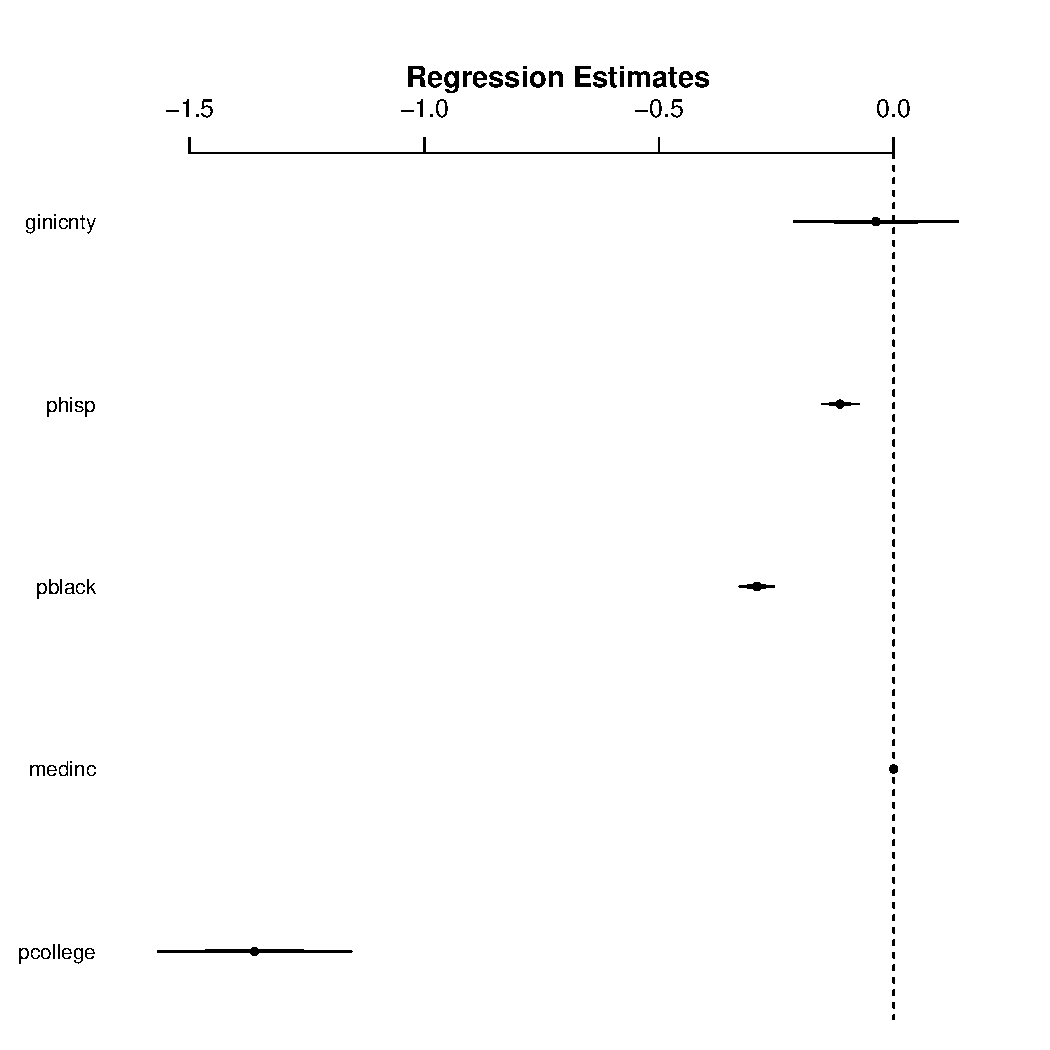
\includegraphics[width=\maxwidth]{figure/unnamed-chunk-9-1} 

\end{knitrout}

That was too easy, so here's another plot

\begin{knitrout}
\definecolor{shadecolor}{rgb}{0.969, 0.969, 0.969}\color{fgcolor}\begin{kframe}
\begin{alltt}
\hlstd{pd} \hlkwb{<-} \hlkwd{melt}\hlstd{(est_3)} \hlopt \hlkwd{filter}\hlstd{(Var2} \hlopt{!=} \hlstr{"(Intercept)"}\hlstd{)} \hlopt
  \hlkwd{dcast}\hlstd{(Var2} \hlopt{~} \hlstd{Var1)}
\hlkwd{ggplot}\hlstd{(}\hlkwc{data} \hlstd{= pd)} \hlopt{+}
  \hlkwd{geom_pointrange}\hlstd{(}\hlkwd{aes}\hlstd{(}\hlkwc{x} \hlstd{= Var2,} \hlkwc{y} \hlstd{= `50%`,} \hlkwc{ymin} \hlstd{= `2.5%`,} \hlkwc{ymax} \hlstd{= `97.5%`))} \hlopt{+}
  \hlkwd{geom_hline}\hlstd{(}\hlkwd{aes}\hlstd{(}\hlkwc{yintercept} \hlstd{=} \hlnum{0}\hlstd{),} \hlkwc{linetype} \hlstd{=} \hlstr{"dotted"}\hlstd{)} \hlopt{+}
  \hlkwd{coord_flip}\hlstd{()} \hlopt{+} \hlkwd{theme_bw}\hlstd{()} \hlopt{+}
  \hlkwd{labs}\hlstd{(}\hlkwc{x} \hlstd{=} \hlstr{""}\hlstd{,} \hlkwc{y} \hlstd{=} \hlstr{"Regression Coefficients"}\hlstd{)}
\end{alltt}
\end{kframe}
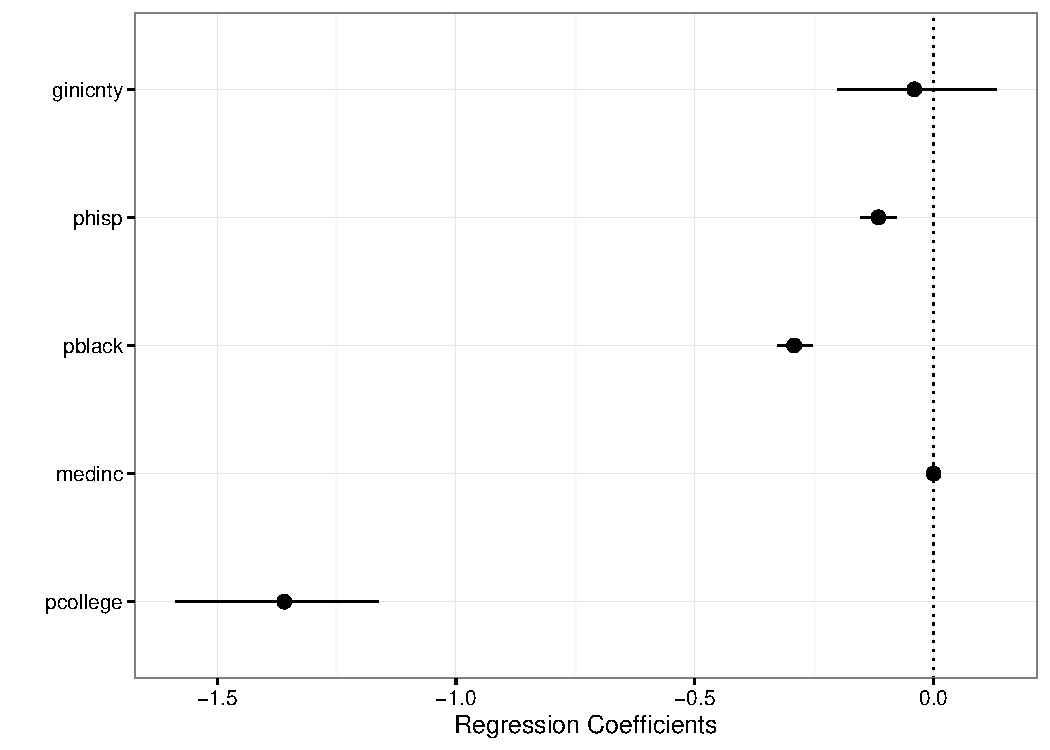
\includegraphics[width=\maxwidth]{figure/unnamed-chunk-10-1} 

\end{knitrout}


\end{document}
